\documentclass[10pt,conference]{IEEEtran}
\usepackage{cite}
\usepackage{amsmath,amssymb,amsfonts}
\usepackage{graphicx}
\usepackage{textcomp}
\usepackage{xcolor}
\usepackage{tikz}
\usepackage{array}
\usepackage[hidelinks]{hyperref}
\usetikzlibrary{positioning,arrows.meta,shapes.geometric}
\pagestyle{plain}
\definecolor{hwcolor}{RGB}{220,235,248}
\definecolor{swcolor}{RGB}{243,243,243}

% Compact IEEE-compliant float/display spacing; body and author fonts remain unchanged.
\setlength{\textfloatsep}{5pt plus 1pt minus 1pt}
\setlength{\floatsep}{4pt plus 1pt minus 1pt}
\setlength{\intextsep}{4pt plus 1pt minus 1pt}
\setlength{\abovedisplayskip}{3pt plus 1pt minus 1pt}
\setlength{\belowdisplayskip}{3pt plus 1pt minus 1pt}
\setlength{\abovedisplayshortskip}{2pt plus 1pt minus 1pt}
\setlength{\belowdisplayshortskip}{2pt plus 1pt minus 1pt}
\setlength{\parskip}{0pt}

\begin{document}

\title{Development of a 60-Gigahertz Millimeter-Wave Vital Signs Monitoring System Using ESP32 for Disaster Aid Management}

\author{\IEEEauthorblockN{Lemuel Blaya\textsuperscript{1}}
\IEEEauthorblockA{\textit{Electronics Engineering Program} \\
\textit{College of Engineering Education}\\
\textit{University of Mindanao}\\
Matina, Davao City, Philippines \\
l.blaya.551860@umindanao.edu.ph \\
{\scriptsize ORCID: 0009-0008-6562-9201}}
\and
\IEEEauthorblockN{Angelo Diaz\textsuperscript{1}}
\IEEEauthorblockA{\textit{Electronics Engineering Program} \\
\textit{College of Engineering Education}\\
\textit{University of Mindanao}\\
Matina, Davao City, Philippines \\
a.diaz.552518@umindanao.edu.ph \\
{\scriptsize ORCID: 0009-0002-2311-6412}}
\and
\IEEEauthorblockN{Blessie Angelie Mugat\textsuperscript{1}}
\IEEEauthorblockA{\textit{Electronics Engineering Program} \\
\textit{College of Engineering Education}\\
\textit{University of Mindanao}\\
Matina, Davao City, Philippines \\
b.mugat.560558@umindanao.edu.ph \\
{\scriptsize ORCID: 0009-0009-1803-689X}}
}

\maketitle
\thispagestyle{plain}

\section{INTRODUCTION}
Earthquakes routinely bury or trap survivors beneath collapsed structures, where conventional contact-based vital-sign checks are impossible and rescuers must decide, under severe time pressure, which locations are worth the risk and labor of extraction. Davao City lies near active fault systems and has documented seismic vulnerability compounding its exposure to riverine flooding; the Department of Social Welfare and Development monitored 49{,}307 displaced individuals across 200 evacuation centers during the 2024 Mindanao floods, and post-earthquake urban search-and-rescue (USAR) operations in the Philippines face comparable congestion and time-critical triage demands \cite{jolly2024,avelino2024,marquez2024}. A portable, non-contact sensor that can indicate whether a living person is present behind rubble or a partition, without requiring rescuers to make physical contact or enter unstable voids, could shorten the search phase and reduce responder risk during the survival-critical first hours after collapse.

Non-contact vital-sign sensing exploits the fact that a radar signal reflected from the chest wall accumulates a phase shift proportional to sub-millimeter displacement, since the round-trip phase of a reflected electromagnetic wave is $\Delta\phi = 4\pi d/\lambda$ for a target displacement $d$ at wavelength $\lambda$; because phase sensitivity to a fixed physical displacement scales inversely with wavelength, this relation is the electromagnetic-theory anchor for why a mmWave carrier is preferred over lower-frequency radio sensing for chest-wall motion \cite{alizadeh2019,zhang2023}. Among the mmWave bands used for radar sensing, 24~GHz, 60~GHz, and 77~GHz are the most common; 77~GHz is predominantly reserved for automotive radar and subject to region-specific regulatory restriction in non-automotive human-sensing contexts, while 24~GHz operates in a less restricted band but has a proportionally longer wavelength, yielding lower phase sensitivity per unit chest-wall displacement than 60~GHz for an equivalent measurement configuration \cite{infineon2026}. A direct comparison of 24~GHz and 77~GHz FMCW radars for breathing and heart-rate extraction found that neither phase sensitivity nor bandwidth alone determined which band performed better, indicating that the choice of band is a design trade-off rather than a strictly dominant option, and separately noted that 24~GHz and 77/79~GHz systems incur higher design and development cost from heterojunction-technology components \cite{singh2022}. The 60~GHz band additionally falls within an unlicensed industrial-scientific-medical (ISM) allocation in most regions, avoiding the automotive-specific certification burden associated with 77~GHz, while its shorter wavelength provides finer range resolution than 24~GHz for the same signal bandwidth \cite{infineon2026}. These characteristics motivate this study's use of a 60~GHz module as a practical balance of phase sensitivity, regulatory accessibility, and component cost for a student-built, low-cost prototype. Reviews identify 60~GHz frequency-modulated continuous-wave (FMCW) radar as suitable for device-free monitoring because its short wavelength provides fine phase sensitivity to chest displacement \cite{tahernejad2024,shastri2022}. Controlled studies have reported respiratory-rate errors near 1~breath/min and reliable extraction in complex scenes \cite{chen2024,yang2025,zhang2026}; however, gross motion, rubble occlusion, and increasing standoff distance can dominate or attenuate chest-wall displacement, motivating missing-data, signal-processing, and learned artifact-control methods \cite{qiao2025,xu2024,fusco2025}. Despite these advances, evidence remains insufficient on whether a low-compute, auditable model can refine HR and RR from the small, heterogeneous, per-window feature sets available to a constrained embedded prototype, at ranges relevant to rubble search (beyond the 1~m typically reported in bench studies), without relying on an external computer. This unresolved implementation-and-validation gap motivates the evaluation of gradient-boosted regression (GBR), which is well suited to modest tabular datasets and can support deterministic embedded inference \cite{grinsztajn2022,shwartzziv2022}.

Edge implementation is increasingly feasible because optimized extraction and TinyML pipelines can operate on microcontroller-class hardware \cite{gao2022,yahyati2025,orsag2023}. Prior systems demonstrate real-time radar monitoring, operation under interference, and sensor fusion \cite{marty2023,kawasaki2023,tanna2023}, while Philippine studies show local mmWave capability \cite{herrera2023,ilagan2023}. Nevertheless, the cited literature does not establish a self-contained MR60BHA2--ESP32-C6 prototype that simultaneously uses only manufacturer-documented UART outputs \cite{seeed_mr60bha2}, performs all processing and inference without an external computer, and quantifies accuracy, valid-output rate, failure modes, and false alarms across controlled distance and obstruction configurations extending to distances relevant for locating a person beyond arm's reach in rubble.

Accuracy degradation with distance and obstruction is not a peripheral concern for this application: a false negative (failing to detect a living, breathing victim) can cost a life if a viable location is skipped, while a false positive (alerting on an empty void) diverts scarce rescue effort from other sites. The consequence of falling short of a 90\% accuracy target is therefore not merely a lower headline number but a specific, discussable operational risk that this study will quantify and report rather than assume away.

The general objective of this study is to design, build, integrate, and test an ESP32-based 60~GHz non-contact vital-sign monitoring prototype intended to assist earthquake search-and-rescue triage. Specifically, the study will \textbf{design} the radar-sensing, temperature-sensing, embedded-inference, and alert subsystems, including a printed-circuit-board (PCB) layout for the sensor--microcontroller interconnect and power distribution; \textbf{build} the prototype hardware enclosure and PCB, evaluating a handheld-scanner form factor against a tripod-mounted form factor through a documented trade-off analysis; \textbf{integrate} the MR60BHA2 radar, XIAO ESP32-C6, MLX90614 temperature sensor, display, buzzer, and GBR inference pipeline into a single operating firmware and hardware unit; and \textbf{test} the integrated prototype's RR and HR accuracy, agreement, and valid-output rate against human reference methods at 0.6, 0.8, 1.0, 2.0, and 3.0~m, without and with a cardboard obstruction, characterizing how accuracy and coverage change as distance increases beyond 1~m.

The study will contribute a portable validation prototype for disaster-response research and support the University of Mindanao priority on Disaster Risk Reduction and Management \cite{um2022}. Its direct beneficiaries are structured-collapse search-and-rescue teams (e.g., Philippine USAR-trained personnel and local disaster-response units) who require a low-cost, rapid triage aid; evacuation-center medical staff who face repeated contact-based screening burdens; and displaced residents and structural-collapse survivors, whose exposure to delayed detection or unnecessary physical handling during triage may be reduced. The study will report measurement uncertainty, repeatability, valid-output rate, failure conditions, and component cost as outcomes rather than presume field or diagnostic performance.

The study will be limited to one prototype and a controlled, minimal-risk validation involving healthy adults aged 18--40 standing in for occluded or distant subjects under laboratory conditions; it will not involve live rubble burial, structural collapse simulation with debris loading, or clinical patients. RR will be the primary outcome, while temperature and HR will be exploratory. The study will exclude diagnosis, clinical-patient testing, simultaneous multi-subject tracking, multiple-posture evaluation, ambulatory or long-range (beyond 3~m) operation, and regulatory certification.

\section{MATERIALS AND METHODS}

\subsection{Research Design}
The study will use a developmental research design, appropriate because the primary output is a working prototype system evaluated against its own design specifications and human-reference measurements rather than a comparison between pre-existing treatment groups \cite{richey2007}. The developmental component will design, build, and integrate the MR60BHA2 radar, XIAO ESP32-C6, MLX90614 sensor, display, buzzer, power source, firmware, and GBR inference into a single prototype. Following non-human functionality checks and UMERC certification, the integrated prototype will undergo a controlled bench evaluation across five distances (0.6, 0.8, 1.0, 2.0, and 3.0~m) under no-cardboard and cardboard conditions with consenting adult volunteers standing in for occluded subjects.

\subsection{Conceptual Framework}
The Input-Process-Output framework in Fig.~\ref{fig:ipo} represents the relation among sensing, edge processing, and triage output. Manufacturer-exposed radar data and infrared temperature enter the ESP32-C6; filtering, spectral feature extraction, GBR refinement, artifact screening, and decision logic produce displayed measurements and alerts.

\begin{figure}[!ht]
\centering
\resizebox{0.92\columnwidth}{!}{%
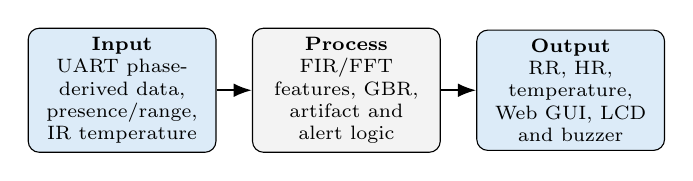
\begin{tikzpicture}[
box/.style={draw,rounded corners,minimum width=2.35cm,minimum height=1.45cm,align=center,text width=2.15cm,font=\scriptsize},
arr/.style={-Latex,thick}]
\node[box,fill=hwcolor] (i) {\textbf{Input}\\UART phase-derived data,\\presence/range, IR temperature};
\node[box,fill=swcolor,right=0.45cm of i] (p) {\textbf{Process}\\FIR/FFT features, GBR,\\artifact and alert logic};
\node[box,fill=hwcolor,right=0.45cm of p] (o) {\textbf{Output}\\RR, HR, temperature,\\Web GUI, LCD and buzzer};
\draw[arr] (i)--(p); \draw[arr] (p)--(o);
\end{tikzpicture}}
\caption{Conceptual framework and edge-processing flow.}
\label{fig:ipo}
\end{figure}

\subsection{Hardware Design and Development}
\textit{Design approach and tools:} The printed-circuit-board interconnect between the MR60BHA2 radar, the XIAO ESP32-C6, the MLX90614 temperature sensor, and the power-management components will be designed using KiCad, an open-source electronic-design-automation (EDA) suite, chosen over proprietary alternatives (e.g., Eagle, Altium) for its zero licensing cost, active community libraries for common breakout modules, and Gerber-file export compatible with both local and overseas low-volume PCB fabrication services. The board will be laid out as a single carrier PCB that exposes UART, I2C, and power headers for the radar and temperature modules rather than relying on loose jumper wiring, reducing intermittent-connection failures during repeated field-style handling and providing a repeatable, documentable hardware baseline for subsequent iterations.

\textit{Firmware and software stack:} Firmware will be written in C/C++ using the Arduino core for the ESP32-C6, selected over MicroPython for its lower runtime overhead and more predictable timing on memory-constrained microcontrollers, which matters for maintaining consistent UART sampling and windowed feature extraction \cite{orsag2023}. The GBR inference pipeline will be trained offline in Python (scikit-learn) and the locked, trained ensemble will be translated into C branch-comparison code for on-device inference, avoiding a floating-point ML runtime dependency on the microcontroller. A lightweight local web GUI, served directly from the ESP32-C6, will mirror the LCD/buzzer output for a rescuer viewing the device from a paired phone or tablet without requiring external connectivity.

\textit{Enclosure fabrication:} The prototype enclosure will be produced using fused-deposition-modeling (FDM) 3D printing in PETG or ABS filament, selected over laser-cut acrylic or off-the-shelf project boxes because FDM printing allows iterative dimensional adjustment as the PCB and battery layout are refined, is inexpensive at low volume, and can be reprinted quickly if a design revision is needed after the trade-off analysis below. Laser-cut acrylic remains a documented fallback if print-bed size or wall-strength requirements exceed what the available FDM printer can reliably produce.

\subsection{Hardware Form-Factor Trade-off Analysis}
Two candidate form factors were considered for the assembled prototype, and this study will document both rather than commit to a single design prior to bench testing, since the better choice depends on results not yet available at the proposal stage.

\textit{Handheld scanner.} A handheld unit, gripped and aimed by a rescuer, offers rapid repositioning between multiple rubble-void locations and does not require a stable mounting surface, which may not exist amid collapsed structural debris. Its principal disadvantage is that hand tremor and micro-motion during 150-s measurement window can introduce phase noise indistinguishable from chest-wall displacement, degrading RR/HR estimation particularly at the longer 2--3~m ranges where signal amplitude is already attenuated.

\textit{Tripod-mounted unit.} A small tripod or clamp-mounted unit eliminates operator hand-motion artifact and provides a fixed, repeatable standoff distance and boresight angle, which is preferable for the controlled bench validation itself and for any location where the rescuer can pause. Its disadvantage is reduced repositioning speed between candidate rubble voids and a dependency on a stable placement surface or clamp point that may not always be available at a collapse site.

Across six comparison criteria, the handheld scanner offers high repositioning speed, higher motion-artifact risk from operator tremor, low standoff repeatability, no dependency on a mounting surface, lower suitability for controlled bench validation, and higher suitability for rapid multi-void search; the tripod-mounted unit offers low repositioning speed, low motion-artifact risk because the sensor is fixed, high standoff repeatability, a dependency on a stable mounting point, higher suitability for controlled bench validation, and lower suitability for rapid multi-void search. Because the two designs trade positioning speed against measurement stability, and because the validation trials in this study will be conducted under controlled bench conditions where a fixed standoff is achievable, the tripod-mounted configuration will be used for the accuracy-validation trials reported here, while the handheld configuration is retained as a field-deployment variant for future work; the final field-deployable form factor is left to the panel's judgment and later design iterations informed by the distance/accuracy results in Section~III.

\subsection{Materials and Resources}
The prototype will integrate a Seeed MR60BHA2 60~GHz radar module, which provides documented UART presence/range, phase-derived waveform, and built-in HR/RR outputs \cite{seeed_mr60bha2}; a Seeed XIAO ESP32-C6 microcontroller (512~KB SRAM), which will ingest the UART frames, derive spectral features, execute the locked GBR model, and drive the interface; and a MLX90614 non-contact infrared sensor, which will provide exploratory single-point skin-surface temperature during unobstructed trials only, since infrared measurement requires direct line of sight to the target. A 20$\times$4 character LCD, an active buzzer, and the ESP32-hosted web GUI described above will together form the measurement-display and audio-visual alert output. A 10{,}000~mAh power bank will supply portable 5-V power for bench and field-style operation. The obstruction condition will use a single-wall corrugated kraft-fiberboard panel of nominal 3~mm thickness, representing a lightweight, reproducible, nonmetallic partition or packed relief supply rather than dense structural rubble. Reference measurements for validation will be obtained from a calibrated infrared thermometer, a pulse oximeter, and a dual-observer full-trial respiration count, as detailed in Section~II-F.

\begin{figure}[!ht]
\centering
\resizebox{0.76\columnwidth}{!}{%
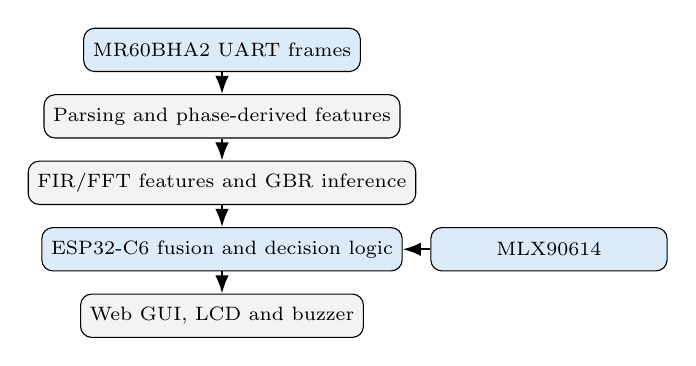
\begin{tikzpicture}[
block/.style={draw,rounded corners,minimum width=3.0cm,minimum height=0.55cm,align=center,font=\scriptsize},
arr/.style={-Latex,thick},node distance=0.28cm]
\node[block,fill=hwcolor] (r) {MR60BHA2 UART frames};
\node[block,fill=swcolor,below=of r] (u) {Parsing and phase-derived features};
\node[block,fill=swcolor,below=of u] (f) {FIR/FFT features and GBR inference};
\node[block,fill=hwcolor,below=of f] (e) {ESP32-C6 fusion and decision logic};
\node[block,fill=hwcolor,right=0.35cm of e] (t) {MLX90614};
\node[block,fill=swcolor,below=of e] (l) {Web GUI, LCD and buzzer};
\draw[arr](r)--(u); \draw[arr](u)--(f); \draw[arr](f)--(e); \draw[arr](t)--(e); \draw[arr](e)--(l);
\end{tikzpicture}}
\caption{Hardware integration and firmware chain.}
\label{fig:architecture}
\end{figure}

Fig.~\ref{fig:architecture} illustrates how these components are wired together in operation. The MR60BHA2 will continuously stream its documented UART frames to the ESP32-C6, which will parse the phase-derived waveform and pass it through FIR/FFT feature extraction and the locked GBR inference stage. In parallel, the MLX90614 will report skin-surface temperature to the same fusion and decision-logic routine running on the ESP32-C6. That routine will combine the GBR-refined RR/HR estimates, the temperature reading, and the frozen artifact/alert rules into a single decision, which will then be pushed simultaneously to the on-board LCD, the buzzer, and the locally hosted web GUI so a rescuer can read the result either directly on the device or on a paired screen.

\begin{figure}[!ht]
\centering
\IfFileExists{figure3.png}{%
\includegraphics[width=0.66\columnwidth,height=0.12\textheight,keepaspectratio]{figure3.png}%
}{%
\fbox{\parbox[c][0.095\textheight][c]{0.62\columnwidth}{\centering\scriptsize Insert \texttt{figure3.jpg}: assembled prototype and labeled components.}}%
}
\caption{Proposed prototype assembly.}
\label{fig:prototype}
\end{figure}

Fig.~\ref{fig:prototype} shows the proposed physical assembly. The MR60BHA2 radar and MLX90614 temperature sensor will be mounted at the forward face of the enclosure, oriented toward the target with an unobstructed sensing window. The XIAO ESP32-C6 and its carrier PCB will sit immediately behind the sensor face, connecting to both modules over short, fixed header runs to minimize wiring flex and intermittent-contact risk. The LCD and buzzer will be mounted on the operator-facing side, and the 10{,}000~mAh power bank will occupy the rear compartment, connected by a short USB lead so it can be swapped without disassembling the sensor housing. The complete enclosure will be produced by FDM 3D printing as described in Section~II-C and will be evaluated in both the handheld and tripod-mounted configurations described in Section~II-D, with the tripod-mounted configuration used for the reported validation trials.

\subsection{Methods and Procedures}

\textit{Implementation of Objective 1---design:} The PCB schematic will be entered in KiCad by first defining the power-supply net (5-V input from the power bank, regulated as required by the ESP32-C6 and sensor modules), then placing the MR60BHA2 UART header, the MLX90614 I2C header, and the ESP32-C6 module footprint, and finally routing signal and power traces with ground-plane pours to reduce noise coupling into the radar's low-level IF signal path. The schematic will be reviewed against each module's datasheet pinout before layout to avoid connector mismatches. A single-sided or two-layer board will be targeted to keep fabrication cost low and lead time short, consistent with the prototype's iterative development timeline. The design will be validated first through a KiCad electrical-rules check (ERC) and then, prior to committing to fabrication, through a breadboard or perfboard bring-up of the same net list using jumper wires, so that any wiring error is caught before it is committed to an ordered PCB. Once the breadboard bring-up confirms correct sensor communication, Gerber files will be exported and submitted to a low-volume PCB fabrication service.

\textit{Implementation of Objective 2---build:} The fabricated PCB will be populated by hand-soldering the ESP32-C6, MR60BHA2, and MLX90614 headers, followed by continuity testing of each net with a multimeter before power is first applied. In parallel, the enclosure will be modeled in a parametric CAD tool (e.g., Fusion 360 or FreeCAD) sized to the populated PCB, the 10{,}000~mAh power bank, the LCD, and the buzzer, and will be produced by FDM 3D printing as described in Section~II-C. Two enclosure variants will be printed to realize the handheld-scanner and tripod-mounted configurations compared in Section~II-D: the handheld variant will include a molded grip and trigger-style activation button, while the tripod-mounted variant will include a standard 1/4-20 tripod-mount insert printed or heat-set into the enclosure base. Both variants will share the same internal PCB and wiring harness so that the sensing and processing hardware does not need to be duplicated or re-soldered between configurations.

\textit{Implementation of Objective 3---integrate:} Firmware integration will proceed in stages rather than as a single combined build, to isolate faults early. First, the MR60BHA2 UART driver will be brought up alone and its raw presence/range/phase output logged to confirm correct frame parsing. Second, the MLX90614 I2C driver will be brought up alone and its temperature readings cross-checked against a handheld reference thermometer. Third, the FIR/FFT feature-extraction stage will be added and its output inspected against the raw phase stream to confirm expected spectral peaks during controlled breathing. Fourth, the locked GBR model, translated to C branch-comparison code as described below, will be integrated as the final stage of the inference pipeline, with its output compared against the FIR/FFT baseline estimate to confirm the residual-correction step is behaving as intended. Fifth, the frozen artifact and alert rules, the LCD/buzzer output driver, and the ESP32-hosted web GUI will be integrated last, so that display and alerting logic cannot mask an upstream sensing or inference fault during development. At each stage, the newly integrated module will be run continuously for at least 30 minutes to check for memory leaks, UART desynchronization, or watchdog resets before proceeding to the next stage; the full integrated firmware will then undergo the 8-hour communication test referenced below prior to human-subject data collection.

\textit{Operational definitions:} \emph{Reference RR} will be defined as the adjudicated full-trial respiration count of two blinded observers converted to breaths/min. \emph{Equivalence} will require the entire 90\% confidence interval for the paired mean difference to fall within $\pm2$~breaths/min at each tested distance. \emph{Valid-output rate} will be the proportion of eligible trials that produce an estimate under the frozen processing rules. \emph{False alarm} will be defined as activation of the frozen alert state during a no-subject trial. The RR equivalence bound and the 90\% accuracy target stated in Section~I are treated as design goals to be tested, not assumed outcomes; where a distance or obstruction condition fails to meet either, the study will report the observed accuracy, the valid-output rate, and the likely operational consequence (missed detection versus false alert) for that configuration rather than omit it.

\textit{Instrument validity and reliability:} Manufacturer checks alone will not be treated as validation. Radar frame rate, range response, continuity, and exposed waveform behavior will be logged at every tested distance; the MLX90614 will be compared with the calibrated reference, and pulse-oximeter signal quality will be checked before each trial. Two RR observers will count independently while blinded to the prototype, pulse oximeter, and each other's reading; absolute-agreement inter-rater reliability and agreement within one breath will be reported. Frozen window-level artifact rules will use phase discontinuity, first-difference magnitude, spectral concentration, broadband energy, range/presence instability, saturation, and minimum usable duration. Repeated measurements, missing-output counts, valid-output rate, reference uncertainty, and an 8-hour communication test will be reported.

\textit{Sampling and participants:} Purposive sampling will recruit 40 healthy adults aged 18--40, targeting at least 38 protocol-complete participants, to stand in for occluded or distant subjects under controlled bench conditions. Exclusions will be known respiratory conditions, BMI above 35, or inability to remain seated and still for 150~s. Recruitment and recording will begin only after UMERC certification; coded identifiers, written consent, withdrawal rights, and approved retention/deletion procedures will be used.

\textit{General trial procedure:} Each participant will complete three 150-s (2.5-min) trials in each of ten randomized radar configurations: no cardboard at 0.6, 0.8, 1.0, 2.0, and 3.0~m, and cardboard at the same five distances, with rest intervals between trials. The 0.6--1.0-m range preserves near-field bench conditions comparable to prior tabletop studies, while the added 2.0 and 3.0~m configurations probe the standoff distances more representative of approaching a partially collapsed structure or a rubble void that cannot be reached directly. The obstruction will be the cardboard panel described in Section~II-E, centered midway, perpendicular to boresight, and large enough to cover the thorax; it represents a simple partition or packed relief supply and is not intended to represent dense structural rubble. Radar, pulse-oximeter, and observer RR data will be acquired in all ten configurations. Temperature will be measured only during unobstructed trials at 0.6~m, since the MLX90614 requires close-range direct line of sight, using a fixed jig after 5-min acclimatization. Seventy-two independent 150-s no-subject trials under one frozen configuration will be conducted for the false-alarm test. Fig.~\ref{fig:testsetup} summarizes the obstructed setup.

\textit{Testing of Objective 4---distance, obstruction, and accuracy:} For every participant and configuration, synchronized radar windows will be processed using the frozen artifact rules and the locked GBR RR and HR models. The median of at least 15 valid windows will form each trial-level estimate, and the mean of at least two valid trials will form each participant-configuration estimate. RR and HR estimates will be paired with the adjudicated dual-observer RR reference and pulse-oximeter HR reference, respectively, and reported per distance using bias, RMSE, MAE, and repeated-measures Bland--Altman limits of agreement, together with the valid-output rate at that distance. Because signal amplitude and phase sensitivity are expected to degrade with range, the study will explicitly test and report whether accuracy and valid-output rate fall below the 90\% target and $\pm2$~breaths/min RR bound at 2.0 and 3.0~m, and will discuss the operational implication of any such shortfall (elevated missed-detection risk at long range versus retained short-range reliability) rather than presenting a single pooled accuracy figure. Temperature agreement at 0.6~m and the no-subject false-alarm rate will be evaluated as in the prior procedure, using repeated-measures Bland--Altman analysis and an exact binomial test with 95\% Clopper--Pearson interval, respectively.

\begin{figure}[!ht]
\centering
\resizebox{0.76\columnwidth}{!}{%
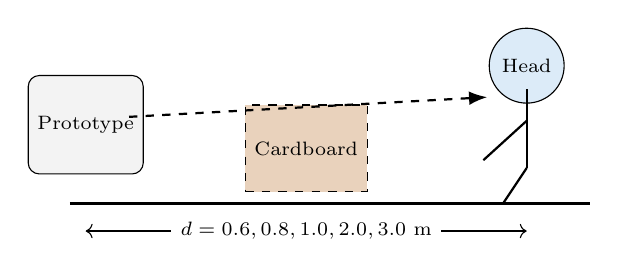
\begin{tikzpicture}[font=\scriptsize,arr/.style={-Latex,thick}]
\draw[thick](0,0)--(6.6,0);
\node[draw,rounded corners,minimum width=1.0cm,minimum height=1.25cm,fill=swcolor] (d) at (0.2,1.0) {Prototype};
\node[draw,dashed,fill=brown!35,minimum width=0.65cm,minimum height=1.1cm] (c) at (3.0,0.7) {Cardboard};
\node[draw,circle,fill=hwcolor,minimum size=0.55cm] (h) at (5.8,1.75) {Head};
\draw[thick](5.8,1.45)--(5.8,0.45); \draw[thick](5.8,1.05)--(5.25,0.55); \draw[thick](5.8,0.45)--(5.5,0);
\draw[arr,dashed](0.75,1.1)--(5.3,1.35);
\draw[<->](0.2,-0.35)--node[fill=white]{$d=0.6,0.8,1.0,2.0,3.0$~m}(5.8,-0.35);
\end{tikzpicture}}
\caption{Cardboard setup; the same distances are tested without cardboard.}
\label{fig:testsetup}
\end{figure}

\textit{GBR development and evaluation:} Training data will come from the UMERC-approved participant trials across all ten configurations. Separate HR and RR models will use synchronized radar features, adjudicated observer RR, and pulse-oximeter HR; temporal lags and rolling statistics will reset at every participant, condition, trial, and sensor-reset boundary. Residual correction will be defined as
\begin{equation}
 e_i=y_i^{\mathrm{ref}}-y_i^{\mathrm{base}},\qquad
 \hat y_i^{\mathrm{GBR}}=y_i^{\mathrm{base}}+\hat e_i.
\end{equation}
\noindent\emph{Legend:} $e_i$ = true residual for observation $i$; $y_i^{\mathrm{ref}}$ = synchronized reference RR or HR; $y_i^{\mathrm{base}}$ = corresponding FIR--spectral baseline estimate; $\hat e_i$ = residual predicted by the GBR; and $\hat y_i^{\mathrm{GBR}}$ = residual-corrected estimate. The module's built-in rate will be an inference-time feature or comparator, not the reference label. Label-, gate-, and alert-derived fields will be blocked by schema checks to prevent leakage from policy/gating logic into the physiology-prediction features. Distance and obstruction condition will be included as explicit categorical features so the model can be evaluated for degradation by range rather than implicitly averaging across it. Nested participant-grouped leave-one-subject-out evaluation will separate tuning from testing; training weights and validation metrics will be participant-balanced. All reported results will use outer-fold predictions only. The locked ensemble will be translated to C branch-comparison code, and flash, RAM, and latency will be measured.

\textit{Statistical analysis:} Thirty-second windows advanced every 5~s will yield 25 predictions per 150-s trial; the median of at least 15 valid windows will form a trial estimate, and the mean of at least two valid trials will form one participant-configuration estimate. A 60-s trial was not retained because it yields only seven highly overlapping windows, allowing settling transients or short artifact intervals to dominate; 150~s provides more physiological cycles and a more stable median while remaining within a manageable period across ten configurations. Per-distance bias, RMSE, MAE, and Bland--Altman limits of agreement will be the primary reported accuracy measures \cite{bland1986,blandaltman2007,addison2024}; correlation will be supplementary, not agreement. Coverage (valid-output rate) and non-output reasons will be reported per distance and obstruction condition so that any coverage loss at longer range is visible rather than absorbed into a pooled statistic. The no-subject criterion will use an exact binomial test and 95\% Clopper--Pearson interval.

\begin{equation}
\operatorname{RMSE}=\sqrt{\frac{1}{n}\sum_{i=1}^{n}(y_i-\hat y_i)^2},\qquad
\operatorname{MAE}=\frac{1}{n}\sum_{i=1}^{n}|y_i-\hat y_i|.
\end{equation}
\noindent\emph{Legend:} $n$ = independent participant or participant-condition estimates; $y_i$ = reference; $\hat y_i$ = prototype estimate.

\begin{equation}
r=\frac{\sum_{i=1}^{n}(x_i-\bar x)(y_i-\bar y)}{\sqrt{\sum_{i=1}^{n}(x_i-\bar x)^2\sum_{i=1}^{n}(y_i-\bar y)^2}}.
\end{equation}
\noindent\emph{Legend:} $r$ = Pearson coefficient; $x_i,y_i$ = paired values; $\bar x,\bar y$ = sample means.

\begin{equation}
\operatorname{MAD}=\operatorname{median}(|X_i-\widetilde X|).
\end{equation}
\noindent\emph{Legend:} $X_i$ = window first-difference or residual; $\widetilde X$ = median. MAD is one component of the frozen artifact rules.

\begin{thebibliography}{31}
\bibitem{jolly2024} S. Jolly, N. Ahmad, and M. Scott, Eds., \textit{Climate-Related Human Mobility in Asia and the Pacific: Interdisciplinary Rights-Based Approaches}. Singapore: Springer Nature, 2024. doi: \url{https://doi.org/10.1007/978-981-97-3234-0}.
\bibitem{avelino2024} B. F. Avelino, C. J. C. Lajos, A. P. Lumantas, and E. R. Gono Jr., ``Disaster preparedness, awareness, and practices of residents within riverine flooding-affected areas in Davao City, Philippines,'' \textit{Eur. J. Educ. Stud.}, vol. 11, no. 4, 2024. doi: \url{https://doi.org/10.46827/ejes.v11i4.5267}.
\bibitem{marquez2024} J. Marquez, ``DSWD: Relief ongoing for Mindanao quake, flooding victims,'' \textit{Philippine Daily Inquirer}, Feb. 5, 2024. [Online]. Available: \url{https://newsinfo.inquirer.net/1900866/fwd-dswd-relief-for-mindanao}.
\bibitem{alizadeh2019} M. Alizadeh, ``FMCW radar system,'' M.S. thesis / technical report, Centre for Intelligent Antenna and Radio Systems (CIARS), University of Waterloo, Jul. 2019. [Online]. Available: \url{https://uwaterloo.ca/centre-for-intelligent-antenna-and-radio-systems/sites/default/files/uploads/documents/fmcwradarsystem.pdf}.
\bibitem{zhang2023} Y. Zhang \textit{et al.}, ``Noncontact cardiac activity detection based on single-channel ISM band FMCW radar,'' \textit{Bioengineering (Basel)}, 2023. [Online]. Available: \url{https://www.ncbi.nlm.nih.gov/pmc/articles/PMC10669854/}.
\bibitem{infineon2026} Infineon Developer Community, ``A comparative analysis of 24~GHz vs. 60~GHz for radar applications,'' Infineon Knowledge Base, 2026. [Online]. Available: \url{https://community.infineon.com/t5/Knowledge-Base-Articles/A-comparative-analysis-of-24-GHz-vs-60-GHz-for-radar-applications/ta-p/1043715}.
\bibitem{singh2022} P. Singh, F. Fioranelli, and O. Aydin Civi, ``Performance comparison of vital signs detection using 24~GHz and 77~GHz radars,'' presented at the \textit{IEEE Radar Conf.}, 2022. [Online]. Available: \url{https://www.researchgate.net/publication/366234130}.
\bibitem{tahernejad2024} A. Tahernejad \textit{et al.}, ``Application of artificial intelligence in triage in emergencies and disasters: a systematic review,'' \textit{BMC Public Health}, vol. 24, p. 3203, 2024. doi: \url{https://doi.org/10.1186/s12889-024-20447-3}.
\bibitem{shastri2022} A. Shastri \textit{et al.}, ``A review of millimeter wave device-based localization and device-free sensing technologies and applications,'' \textit{IEEE Commun. Surveys Tuts.}, vol. 24, no. 3, pp. 1708--1749, 2022. doi: \url{https://doi.org/10.1109/COMST.2022.3177305}.
\bibitem{chen2024} Y. Chen \textit{et al.}, ``A high precision vital signs detection method based on millimeter wave radar,'' \textit{Sci. Rep.}, vol. 14, 2024. doi: \url{https://doi.org/10.1038/s41598-024-77683-1}.
\bibitem{yang2025} X. Yang \textit{et al.}, ``Super-range-resolution respiratory signals detection from multiple targets with single-channel FMCW radar,'' \textit{IEEE Trans. Instrum. Meas.}, vol. 74, 2025. doi: \url{https://doi.org/10.1109/TIM.2025.3553244}.
\bibitem{zhang2026} C. Zhang \textit{et al.}, ``A radar vital signs detection method in complex environments,'' \textit{Sci. Rep.}, vol. 16, p. 2333, 2026. doi: \url{https://doi.org/10.1038/s41598-025-32042-6}.
\bibitem{qiao2025} X. Qiao \textit{et al.}, ``Millimeter-wave radar vital signs measurement with random body movement using missing data model,'' \textit{IEEE Trans. Instrum. Meas.}, vol. 74, 2025. doi: \url{https://doi.org/10.1109/TIM.2025.3547495}.
\bibitem{xu2024} D. Xu, W. Yu, Y. Wang, and M. Chen, ``Vital signs detection in the presence of nonperiodic body movements,'' \textit{IEEE Trans. Instrum. Meas.}, vol. 73, Art. no. 8004816, 2024. doi: \url{https://doi.org/10.1109/TIM.2024.3450071}.
\bibitem{fusco2025} A. Fusco \textit{et al.}, ``Deep learning classifier for robust artifact rejection in FMCW radar vital sensing,'' \textit{IEEE Sensors J.}, vol. 25, 2025. doi: \url{https://doi.org/10.1109/JSEN.2024.3497797}.
\bibitem{grinsztajn2022} L. Grinsztajn, E. Oyallon, and G. Varoquaux, ``Why do tree-based models still outperform deep learning on typical tabular data?'' in \textit{Proc. NeurIPS Datasets and Benchmarks Track}, 2022. [Online]. Available: \url{https://openreview.net/forum?id=Fp7__phQszn}.
\bibitem{shwartzziv2022} R. Shwartz-Ziv and A. Armon, ``Tabular data: Deep learning is not all you need,'' \textit{Information Fusion}, vol. 81, pp. 84--90, 2022. doi: \url{https://doi.org/10.1016/j.inffus.2021.11.011}.
\bibitem{gao2022} Z. Gao \textit{et al.}, ``Real-time non-contact millimeter wave radar-based vital sign detection,'' \textit{Sensors}, vol. 22, no. 19, p. 7560, 2022. doi: \url{https://doi.org/10.3390/s22197560}.
\bibitem{yahyati2025} C. Yahyati \textit{et al.}, ``A systematic review of state-of-the-art TinyML applications in healthcare, education, and transportation,'' \textit{IEEE Access}, vol. 13, 2025. doi: \url{https://doi.org/10.1109/ACCESS.2025.3633575}.
\bibitem{orsag2023} J. Orsag, J. Kalova, and P. Silhavy, ``Performance evaluation of C/C++, MicroPython, Rust and TinyGo programming languages on ESP32 microcontroller,'' \textit{Electronics}, vol. 12, no. 1, p. 143, 2023. doi: \url{https://doi.org/10.3390/electronics12010143}.
\bibitem{marty2023} S. Marty \textit{et al.}, ``Investigation of mmWave radar technology for non-contact vital sign monitoring,'' in \textit{Proc. IEEE MeMeA}, 2023. doi: \url{https://doi.org/10.1109/MeMeA57477.2023.10171940}.
\bibitem{kawasaki2023} R. Kawasaki and A. Kajiwara, ``60~GHz MMW sensor for monitoring driver's vital signs,'' \textit{IEICE Commun. Express}, vol. 12, no. 4, 2023. doi: \url{https://doi.org/10.1587/comex.2022XBL0195}.
\bibitem{tanna2023} R. S. Tanna and C. H. Vithalani, ``IoT-based health monitoring of sports personnel through wearables using machine learning technology,'' 2023. [Online]. Available: \url{https://www.ukdr.uplb.edu.ph/journal-articles/6230}.
\bibitem{herrera2023} J. A. Herrera \textit{et al.}, ``Millimeter wave radar sensing technology for Filipino Sign Language recognition,'' in \textit{Pervasive Computing Technologies for Healthcare}, vol. 488. Springer, 2023, pp. 291--306. doi: \url{https://doi.org/10.1007/978-3-031-34586-9_19}.
\bibitem{ilagan2023} L. C. Ilagan and E. P. Dadios, ``Wireless sensor network using millimeter wave for chemical detection,'' in \textit{Proc. IEEE ECICE}, 2023, pp. 269--271. doi: \url{https://doi.org/10.1109/ECICE59523.2023.10382978}.
\bibitem{seeed_mr60bha2} Seeed Studio, ``Getting started with 60GHz mmWave Breathing and Heartbeat Detection Sensor Kit with XIAO ESP32C6 (MR60BHA2),'' \textit{Seeed Studio Wiki}. [Online]. Available: \url{https://wiki.seeedstudio.com/getting_started_with_mr60bha2_mmwave_kit/}. [Accessed: Jul. 22, 2026].
\bibitem{um2022} University of Mindanao, \textit{Excellence in Research Towards Sustainable Development in Mindanao: Research Agenda 2022--2027}. Davao City, Philippines, 2022.
\bibitem{richey2007} R. C. Richey and J. D. Klein, \textit{Design and Development Research: Methods, Strategies, and Issues}. Mahwah, NJ: Lawrence Erlbaum Associates, 2007.
\bibitem{bland1986} J. M. Bland and D. G. Altman, ``Statistical methods for assessing agreement between two methods of clinical measurement,'' \textit{Lancet}, vol. 327, no. 8476, pp. 307--310, 1986. doi: \url{https://doi.org/10.1016/S0140-6736(86)90837-8}.
\bibitem{blandaltman2007} J. M. Bland and D. G. Altman, ``Agreement between methods of measurement with multiple observations per individual,'' \textit{J. Biopharm. Statist.}, vol. 17, no. 4, pp. 571--582, 2007. doi: \url{https://doi.org/10.1080/10543400701329422}.
\bibitem{addison2024} P. S. Addison \textit{et al.}, ``Non-contact monitoring of inhalation-exhalation (I:E) ratio in non-ventilated subjects,'' \textit{IEEE J. Transl. Eng. Health Med.}, vol. 13, pp. 1--12, 2024. doi: \url{https://doi.org/10.1109/JTEHM.2024.3496196}.
\end{thebibliography}

\end{document}
